% !TEX root = ../Thesis.tex
% !TEX spellcheck = en-US

\chapter{Leaving the physical world}
\label{ch:leavingthephysicalworld}

This chapter addresses which of the two technologies---emulation or simulation---is a better answer to the problem presented in the introduction:
in education, how can we avoid the usage of laboratories cluttered with network gear.
We start by showing what are the fundamental characteristics that set them apart, and also that emulation has its intrinsic advantages over simulation with regard to the above stated problem.

Finally, it offers a brief overview of the state of the art on the topic of virtualization, which supports, in its lighter or more resource-intensive forms, most of computer network emulators today.

% Section "Emulation and simulation"
\section{Emulation and simulation}
\label{sec:leavingemulationandsimulation}

Providing a precise definition, or ``definition framework,'' for distinguishing simulators from emulators and why \emph{emulation} (as opposed to \emph{simulation}) is the focus of this dissertation is paramount.
In the literature, Wikipedia, or common dictionaries, there are contradictory definitions, overlapping concepts, and, in general, a vague distinction between the two is presented~\cite{netsimoremu}. % TODO find and insert citations
That is why, rather than universally establishing what an emulator and a simulator are, it is intended that when, throughout this text, software package $A$ is an emulator and $B$ is a simulator in this or that sense, the reader can know without ambiguity what is meant.

% \begin{figure}
%   \centering
%   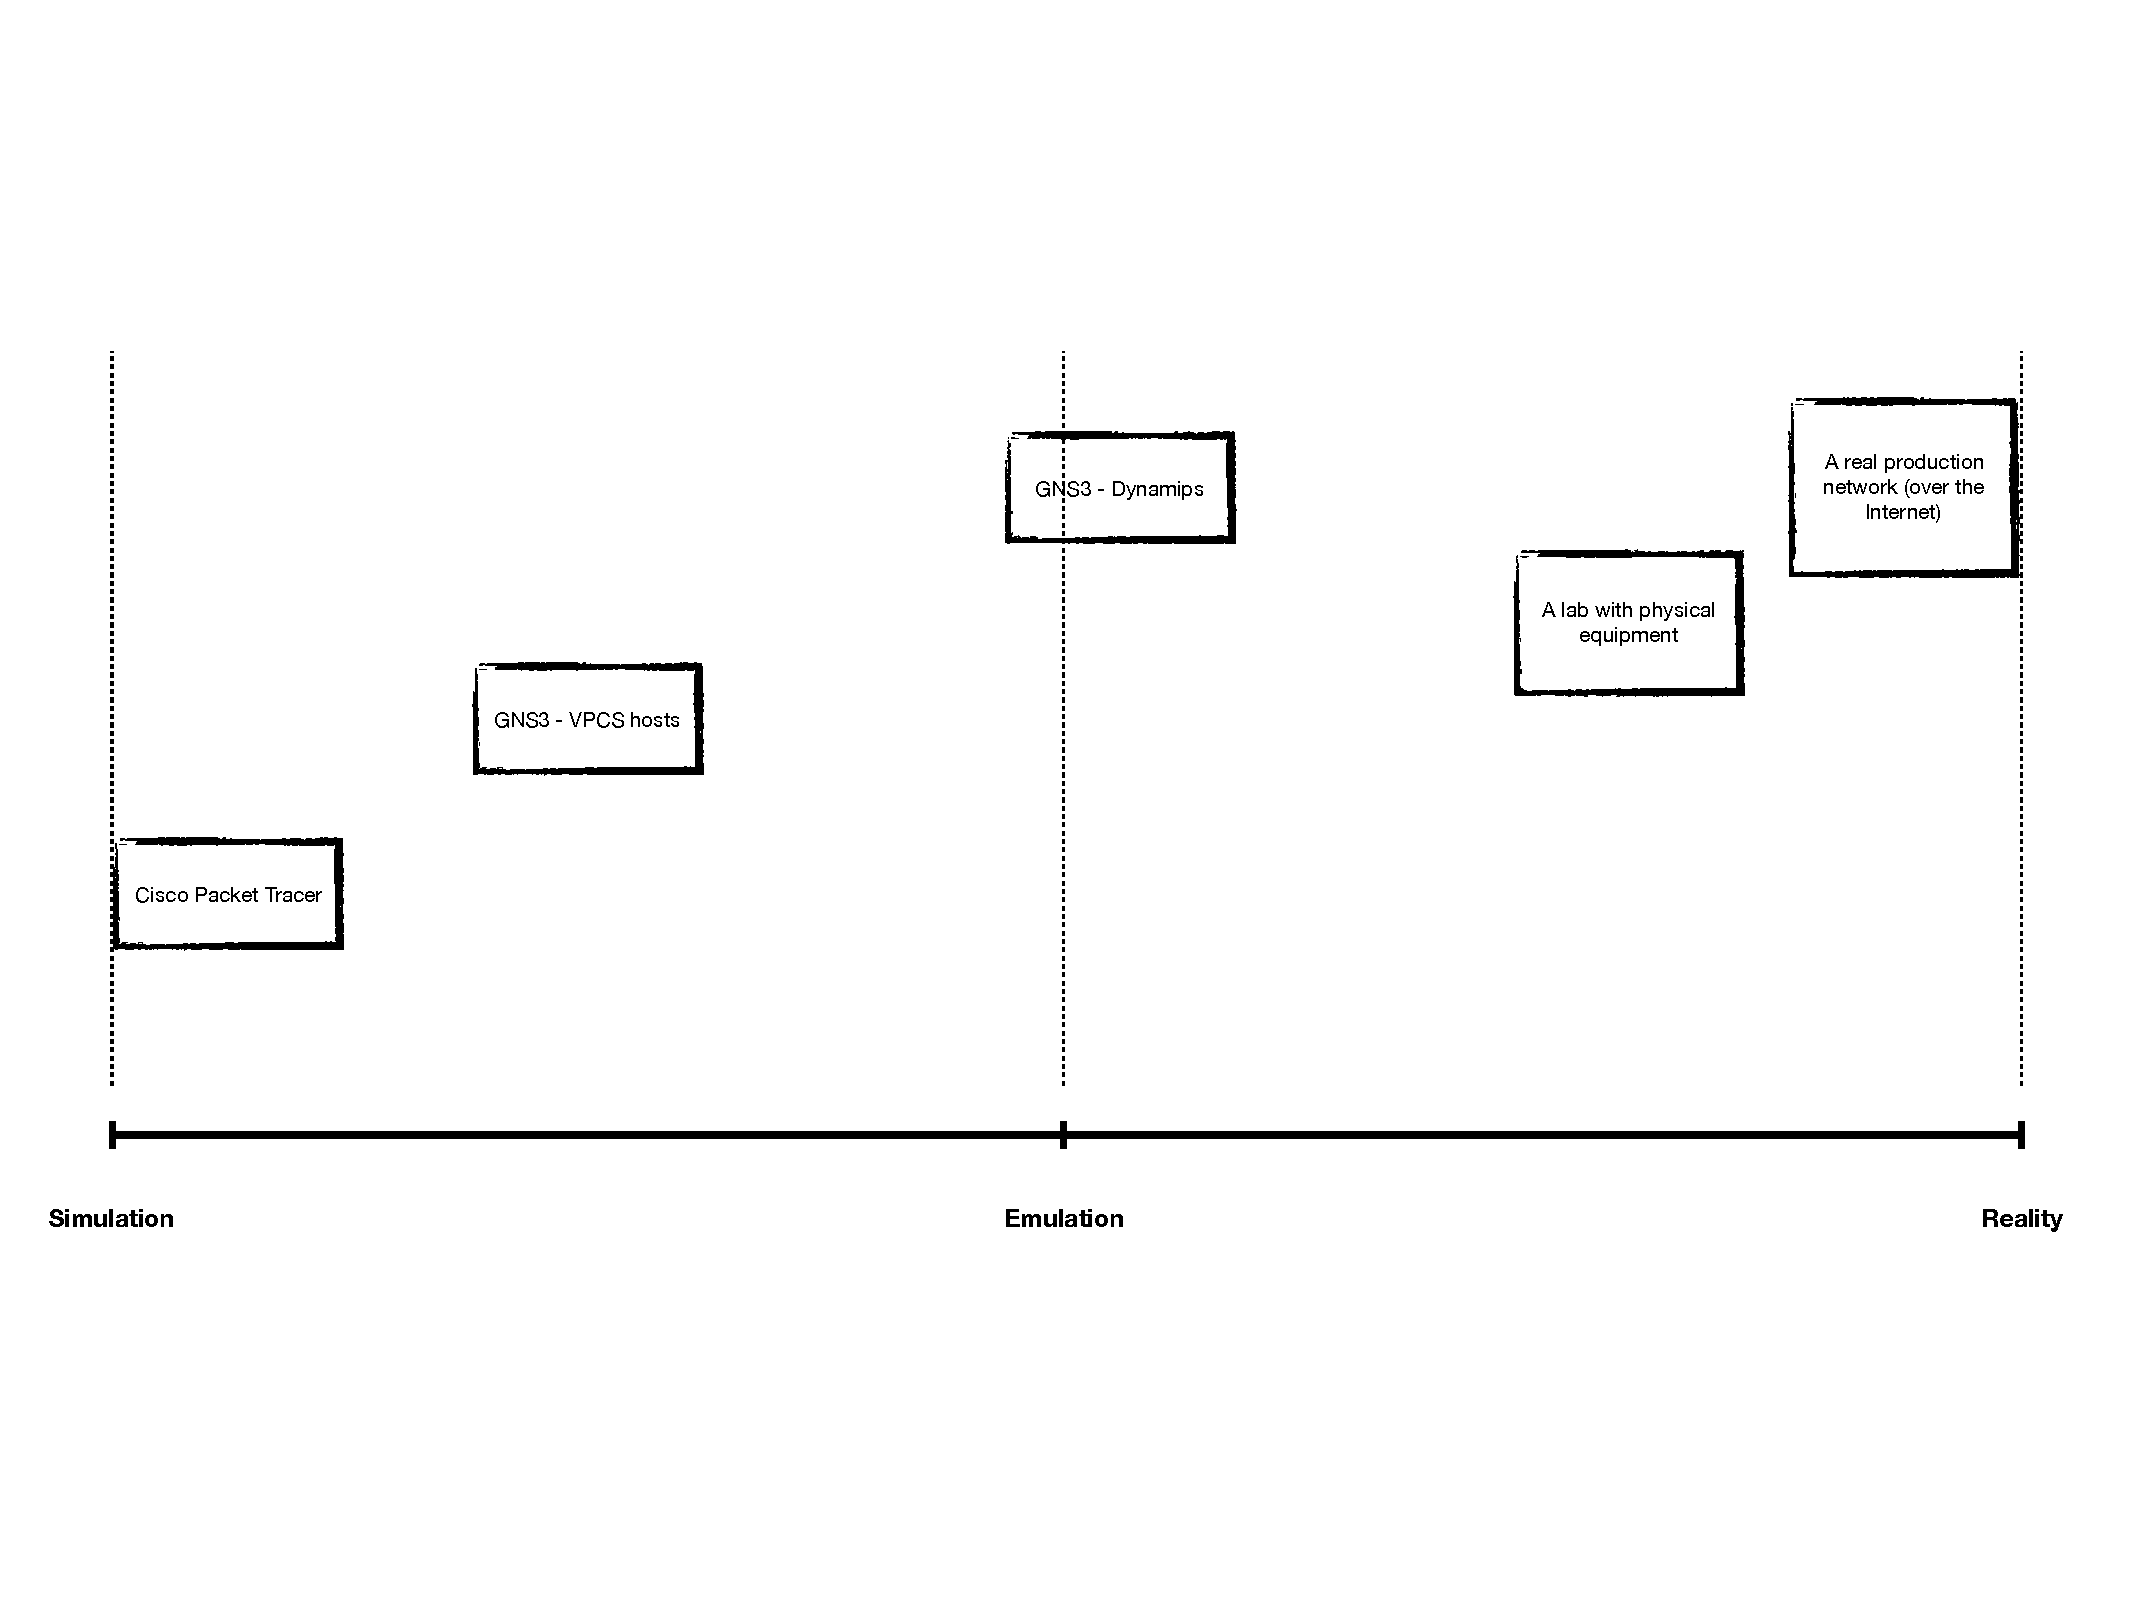
\includegraphics[width=0.8\textwidth]{emulationvsreality}
%   \caption{Simulation vs emulation vs reality}
%   \label{fig:emulationvsreality}
% \end{figure}

Before pointing out the differences between emulators and simulators, it is important to say what both have in common: they are ways of providing students, researches, developers, administrators, or any professional that works with computer networks with an alternative to the real network that is being studied, for convenience and/or cost effectiveness.
However, a lab with network nodes in an education institution is also different from the reality it is trying to model.
%That idea is exposed in the diagram in figure~\ref{fig:emulationvsreality}.

On one end there is reality---in a lab, factors like amount of nodes, physical length of links (and therefore propagation times) can only be \textbf{simulated}, let alone on an solution that is fully software-based, like the emulators described later in this section.
An anecdote like the 500-mile email~\footnote{The case of the 500-mile email~\cite{500mileemail} was an issue described by a systems administrator where e-mails could not be sent to servers further than 500 miles.
The description seemed impossible as e-mail servers (closer) were working, but a hidden configuration---a timeout---rendered a different behavior according to the physical distance between hosts, due to round-trip times.
} could not be reproduced, without simulating an---then---unknown ``flaw,'' in an emulator consisting in virtual machines running the real software and performing the real operations: the cause of the problem was latency.
On the other end there is full simulation, where nothing is real.

In between, complex solutions like GNS3, which is presented in great detail in chapter~\ref{ch:gns3}, can offer a mixture, while being mainly emulators in the sense that it consists in an orchestrated set of processes running the real code, and also allowing to simulate aspects of reality like failures in links and delays.

The reason why emulators are specially interesting and are essentially the motivation (\ref{sec:motivation}) of this work, though, is that giving away the lab room with its switches and cables requires to not lose the flexibility it offers to perform all kind of pedagogical exercises, and ``pure'' simulators do not offer by inherent limitation.

%A network simulator is a computer program (or software package) that implements algorithms corresponding to a \textbf{model} of the reality through software components.
In~\cite{netkit-full}, the article presenting Netkit (a tool studied later in this thesis) and the process that led to its inception, which largely overlaps with the present work, there's an interesting paragraph that explains succinctly the difference between simulation and emulation.
Note that these concepts exist for any kind of \emph{system}, of which any computer system, such as computer networks, are only particular instances (emphasis \textbf{not} present in the original document):
\begin{displayquote}
Simulation aims at computing the behavior of a network based on an abstract model that usually ignores many functional details (e.g., message formats, the need for configurations, and the presence of command line interfaces).
This approach is suited for massive performance-oriented experiments and usually produces accurate event timing information.
Emulation aims at accurately reproducing the behavior of a real network in all its functional details and is usually achieved by exploiting as much as possible the same software (or an open version of it) that would be used on real devices.
Although considerably less efficient than simulation and usually inadequate to reproduce timings observed in real network systems, this approach is very effective to capture the wide range of functionalities and behaviors of a real network, and we believe \emph{it is therefore much more suited for didactics than simulation}.
\end{displayquote}
Simulators like ns-3~\cite{ns3} or the OPNET~\cite{introtoopnet} are discrete event simulators~\cite{netsimoremu}.
They enable, through some interface---such as a graphical one---, designing, testing, analyzing, and observing the expected behavior of protocols, nodes, and links according to several parameters. Therefore, it serves as a way to study protocols used across the stack, and possibly even some application layer components can be ``mimicked''.

Even though the usefulness of these tools cannot be questioned, and some like Cisco Packet Tracer~\footnote{\url{https://www.netacad.com/courses/packet-tracer/introduction-packet-tracer}}, also a discrete event simulator~\cite{evaluatingnetsimmethodologicapproach}, are very widely used in the training of professionals in the networks administration and engineering fields~\cite{rolepackettracer}, it is crucial to point out as the distinctive characteristic of simulators, as defined here, the fact that those applications constitute a ``closed'' universe in the sense of only \emph{simulating} events that change the status of internal data structures, but do not implement a real stack of protocols, where every operation that should be performed is, in fact, performed. % TODO this is super "Portuguese in English". Improve

In other words: a network simulator is a black box for the outside, with a set of available inspection and state alteration operations---i.e. that provides the ability to see some aspects of the simulated system and perform some finite set of changes to the simulated environment.
% However, as long as the \emph{implemented} cause-effect behaviors for that set of operations \emph{is coherent} to their real-world counterparts, any kind of ``shortcuts'' inside can be taken.

On the other hand, the definition for an emulator can, therefore, pretty much be inferred from the simulator as its ``complementary.''
Software computer network emulators are solutions that allow, without resorting to the usage of physical equipment (even though sometimes allow for it, if desired) prototyping networks for analysis and study of underlying mechanisms, investigation, and development of new protocols and solutions, etc., thanks to an array of techniques that can span from virtualization and containerization, hardware architecture emulation, and leveraging operating system functionality in multi-process environments.

Unlike the simulators, described earlier, the fact of the traffic being real (at least from a logical standpoint) and that is possible to ``glue'' emulated interfaces with any kind of physical ones detected by the host operating system, offers the possibility of mixing emulated topologies with real topologies, cloud machines, etc.
Besides, since the computational nodes (hosts in the emulated topologies) are in, fact, ``generic'' hosts (nowadays, usually VMs or containers), running real software, the limit in terms of what it is possible to configure, parameterize, implement, or test, for any stack level (from the link to the application layer) is virtually nonexistent.

% end of section leavingemulationandsimulation


% Section "Virtualization tecnologies"
\section{Virtualization Technologies}
\label{sec:leavingvirtualization}

A broad, loose, and multiple-purpose oriented definition of (computer) virtualization can be taken out of the excellent essay that is~\cite{introvirtualization}:
\begin{displayquote}
Virtualization is a framework or methodology of dividing the resources of a computer into multiple execution environments, by applying one or more concepts or technologies such as hardware and software partitioning, time-sharing, partial or complete machine simulation, emulation, quality of service, and many others.
\end{displayquote}

However, to narrow down the definition in this case, we can say that a virtual machine, under  a modern multiprocess OS, is a software-based execution \emph{context} where one or more programs can be run in isolation when observed outside of that context.
The degree by which this isolation is provided varies on different kinds of virtualization.

In full-system virtualization (also called hardware-level virtualization), the aforementioned OS is a specialized one, called hypervisor or \gls{vmm}.
The \gls{vmm} emulates a fully-fledged computer, the \gls{vm}, with CPUs, RAM, peripheral devices (e.g. \glspl{nic}, disks), etc.; therefore the \gls{vm}, indistinguishable from a real machine, can run a standard OS, which is then called the guest OS.
Usually, the term \gls{vm}, without any more information, refers to a full-system virtual machine.

Hypervisors such as, for example, VMware Workstation\footnote{\url{https://www.vmware.com/products/workstation-pro.html}} (and free alternatives, like VirtualBox\footnote{\url{https://www.virtualbox.org}} from Sun, now Oracle) that run along a standard OS such as Windows, macOS, or Linux in the same host and rely on the OS for some operations are called type-II or hosted hypervisors.
Others, such as VMware ESXi, Citrix Xen, Microsoft Hyper-V, Apple's Hypervisor, or KVM (the last three are provided by Windows, macOS, and Linux, respectively~\cite{whatiskvm,applehypervisor,hyperv}) that run stand-alone (ESXi) or rely on the standard OS only for resource management (all other examples), are called type-I, bare metal, or native hypervisors.

In OS-based virtualization, the OS creates separated contexts, called containers, that share the base OS kernel, but run in isolation with regard to other containers.
They are, when compared with \glspl{vm}, less resource hungry, and as such are also designated as a lightweight virtualization technology.

Linux has included in-kernel support for containerization for many years, but there was a recent upsurge in the use of containers as a result of Docker Inc.'s work on a string of technologies that very much simplify the use of containers~\cite{hwswvirt,virtessentials}.
The a schematic depiction of the difference between full-system virtualization and containers is offered in~\ref{fig:docker-vs-vms}, taken from~\cite{dockercontreplacingvms}.

% As~\cite{introvirtualization} describes, full virtual machines was typically a costly thing to do, especially on x86-based machines.
% However, the article is question is quite old.
% Even though there are more lightweight alternatives, presented afterwards, full-blown virtual machines are nowadays lighter, modern x86 processors provide hardware acceleration techniques to make it closer to native as well, and the sheer capacity of commodity hardware is also bigger than ever~\cite{virtualizationcontainerization}.

% However, other solutions exist that provide lower isolation levels (from an implementation standpoint) that can suffice for certain applications, as shown in later chapters. Nowadays, this concept is usually called containers.
% A container is a process running on the host's OS which resorts to technologies like \emph{Cgroups} and \emph{namespaces}, both provided by the Linux kernel, to be able to isolate its child processes from the host's or other containers' processes, namely in aspects of networking.
% However, the kernel is actually the same, which reduces the overhead dramatically~\cite{comparativevmscontainers}.

% A particular container infrastructure, very popular nowadays is Docker, which uses the aforementioned Linux kernel technologies but provides a whole set of tools that make working with containers, pre-defining \emph{images} to run on containerized infrastructure and distributing them, configuring, and even transparently providing a thin Linux virtual machine for non-Linux desktop environments.

% A high-level illustration of the difference between applications running on ``regular,'' full-blown VMs and applications running over Docker (here, Docker represents the full set of OS-functionality and APIs it abstracts to provide a ``container infrastructure'') is offered by figure~\ref{fig:docker-vs-vms}, taken from~\cite{dockercontreplacingvms}.

% Figure fig:docker-vs-vms
\begin{figure}
  \centering
  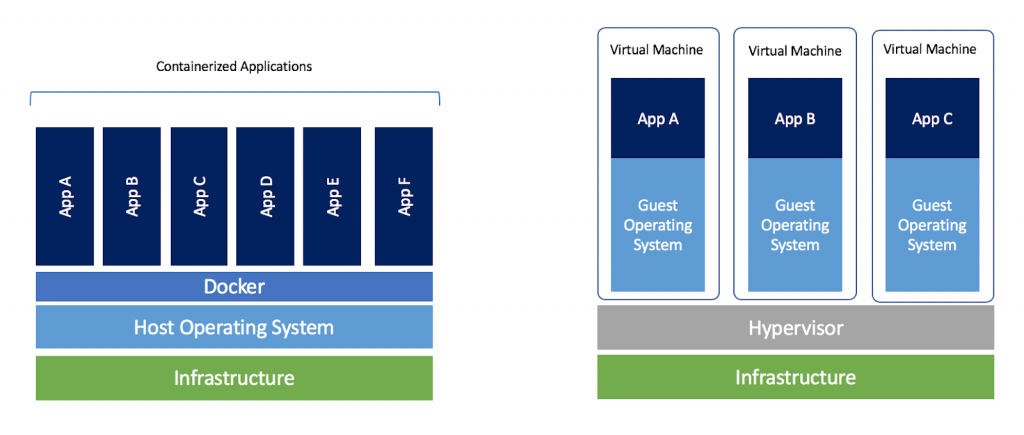
\includegraphics[width=0.8\textwidth]{docker-vs-vms}
  \caption{\textquote{Containers versus Virtual Machines}}
  \label{fig:docker-vs-vms}
\end{figure}


% end of section leavingvirtualizationtechnologies


% Section "Summary"
\section{Summary}
\label{sec:leavingsummary}

In this chapter we presented:
\begin{itemize}
  \item two existing conceptual approaches to replace ``the real thing,'' in the particular case of computer networks, with a virtual alternative by the means of software;
  \item the underlying mechanisms that enable emulation, which is the approach studied in-depth in this dissertation.
\end{itemize}

% end of section exemulsummary


% end of chapter
